% Pre-ambulo
\documentclass[a4paper, 12pt]{abnt}

%\usepackage{hyperref}
\usepackage[english]{babel}
\usepackage[utf8]{inputenc}
\usepackage[T1]{fontenc}
\usepackage{dsfont}
\usepackage{amssymb,amsmath}
\usepackage{multirow}
\usepackage[alf]{abntcite}
\usepackage[pdftex]{color, graphicx}
\usepackage{colortbl}
\usepackage{url}
\usepackage{abnt-alf}
\usepackage{abntcite}
\usepackage{algorithm}
\usepackage{algorithmic}

% Pacotes adicionados
\usepackage{amsthm}
\usepackage{booktabs}
\usepackage{caption}
\usepackage{subcaption}
\usepackage{longtable}
\usepackage{array}
\usepackage{tikz}
\usetikzlibrary{shapes,arrows}
%\usepackage{filecontents,pgfplots}
%\usepackage{pgfplotstable}
\usepackage[inline]{enumitem}
\usetikzlibrary{positioning, arrows}

\usepackage[protrusion=true,expansion=true]{microtype}

\theoremstyle{definition}
\newtheorem{definition}{Definition}[section]
 
\theoremstyle{remark}
\newtheorem*{remark}{Remark}
\usepackage{arydshln}
%\usepackage{alg}

\renewcommand{\theequation}{\arabic{equation}}

% Definicao da lista de simbolos
% \simb[entrada na lista de simbolos]{simbolo}:
% Escreve o simbolo no texto e uma entrada na lista de simbolos.
% Se o parametro opcional e omitido, usa-se o parametro obrigatorio.
\newcommand{\simb}[2][]
{%
	\ifthenelse{\equal{#1}{}}
	{\addcontentsline{los}{simbolo}{#2}}
	{\addcontentsline{los}{simbolo}{#1}}
}
% Para aceitar comandos com @ (at) no nome
\makeatletter 
% \listadesimbolos: comando que imprime a lista de simbolos
\newcommand{\listofsymbols}
{
	\pretextualchapter{List of symbols}
	{\setlength{\parindent}{0cm}
	\@starttoc{los}}
}
% Como a entrada sera impressa
\newcommand\l@simbolo[2]{\par #1}
\makeatother

% Definicao da lista de abreviaturas e siglas
% \abrv[entrada na lista de simbolos]{abreviatura}:
% Escreve a sigla/abreviatura no texto e uma entrada na lista de abreviaturas e siglas.
% Se o parametro opcional e omitido, usa-se o parametro obrigatorio.
\newcommand{\abrv}[2]
{
	\ifthenelse{\equal{#1}{}}
	{\addcontentsline{loab}{abreviatura}{#2}}
	{\addcontentsline{loab}{abreviatura}{#2 \textemdash \ #1}}%
}

% Para aceitar comandos com @ (at) no nome
\makeatletter 
% \listadeabreviaturas: comando que imprime a lista de abreviaturas e siglas
\newcommand{\listadeabreviaturas}
{
	\pretextualchapter{List of abbreviations}
	{\setlength{\parindent}{0cm}
	\@starttoc{loab}}
}
% Como a entrada sera impressa
\newcommand\l@abreviatura[2]{\par #1}
%\newcommand\l@abreviatura[2]{} % Não imprime a entrada, apenas adiciona na tabela
\makeatother

% \listofalgorithms: comando que imprime a lista de algoritmos
\renewcommand{\listalgorithmname}{List of algorithms}

% Hifeniza  o de palavras feita de forma incorreta pelo LaTeX
\hyphenation{PYTHON ou-tros}

\newcommand{\myequation}[2][]
{%
	\ifthenelse{\equal{#1}{}}
	{\addcontentsline{loe}{simb}{#2}}
	{\addcontentsline{loe}{simb}{#1}}
}

% Inicio do documento
\begin{document}

	\frenchspacing
	
	% Capa (arquivo Includes/Capa.tex)
	% Capa
% Prote  o externa do trabalho e sobre a qual se imprimem as informa  es indispens veis 
%   sua identifica  o.

% Especifica  o da capa
\begin{titlepage}
	\begin{center}
		
		% Cabe alho (n o deve ser modificado)
		% Cont m o bras o da Universidade, o logotipo do Departamento, al m dos dados
		% relacionados   vincula  o do aluno (Universidade, Centro, Departamento e Curso)
		\begin{minipage}{2cm}
			\begin{center}
				
\includegraphics[width=1.7cm, height=2.0cm]{Imagens/Brasao-UFRN.jpg}
			\end{center}
		\end{minipage}
		\begin{minipage}{11cm}
			\begin{center}
				\begin{espacosimples}
					{\small \textsc{Federal University of Rio Grande do Norte}			\\
							  \textsc{Center for Exact and Earth Sciences}						\\
\textsc{Bachelor in Computer Science}}
				\end{espacosimples}
			\end{center}
		\end{minipage}
		\begin{minipage}{2cm}
			\begin{center}
				
\includegraphics[width=1.8cm, height=1.5cm]{Imagens/Logotipo-DIMAp.jpg}
			\end{center}
		\end{minipage}
			
		\vspace{6cm}
						
		% T tulo do trabalho
		{\setlength{\baselineskip}%
		{1.3\baselineskip}
		{\LARGE \textbf{Developing a web system for predicting student success using learning analytics}}\par}
			
		\vspace{4cm}
			
		% Nome do aluno (autor)
		{\large \textbf{Lucas Aléssio Anunciado Silva}}
						
		\vspace{7cm}
		
		% Local da institui  o onde o trabalho deve ser apresentado e ano de entrega do mesmo
		Natal-RN\\ September 2021
	\end{center}
\end{titlepage}

	% Folha de rosto (arquivo Includes/FolhaRosto.tex)
	% Folha de rosto
% Cont m os elementos essenciais   identifica  o do trabalho.

% T tulo, nome do aluno e respectivo orientador e filia  o
\titulo{\Large{Developing a web system for predicting student success using learning analytics}}
\autor{Lucas Aléssio Anunciado Silva}
\orientador[Advisor]{\par Isabel Dillmann Nunes, PhD}
\instituicao
{
	Federal University of Rio Grande do Norte -- UFRN 
}
	
% Natureza do trabalho (n o deve ser modificada)
\comentario
{
% 	Monografia de Graduação apresentada ao Departamento de Informática e Matemática Aplicada do 
% 	Centro de Ciências Exatas e da Terra da Universidade Federal do Rio Grande do Norte como
% 	requisito parcial para a obtenção do grau de bacharel em Ciência da Computação.
	Undergraduate Report presented as a
	partial requirement for obtaining the degree of Bachelor in
	Computer Science.
}
		
% Local e data
\local{Natal-RN}
\data{August 2021}
	
\folhaderosto	
	
	% Ficha catalográfica
	\vfill
\begin{figure}[H]
    \centering
    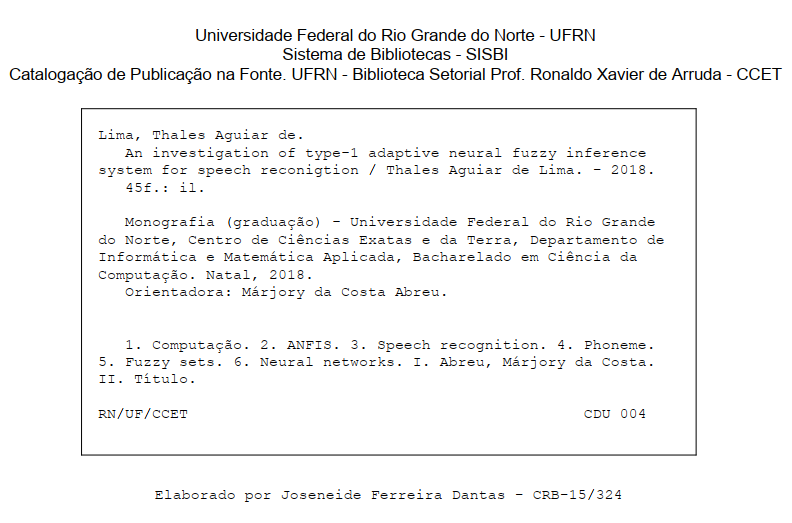
\includegraphics[width=\textwidth]{Imagens/ficha_catalografica.png}
\end{figure}


	
	% Folha de aprovacao (arquivo Includes/FolhaAprovacao.tex)
	% Folha de aprova    o
\begin{folhadeaprovacao}
	\setlength{\ABNTsignthickness}{0.4pt}
	\setlength{\ABNTsignwidth}{10cm}
	
	% Informa    es gerais acerca do trabalho 
	% (nome do autor, t  tulo, institui    o    qual    submetido e natureza)
	\noindent 
% 	Monografia de Graduação sob o título \textit{An Investigation of Type-1 Adaptive Neural Fuzzy Inference System for Speech Reconigtion} apresentada por 
% 	Thales Aguiar de Lima e aceita pelo Departamento de Informática e Matemática Aplicada do
% 	Centro de Ciências Exatas e da Terra da Universidade Federal do Rio Grande do Norte,
% 	sendo aprovada por todos os membros da banca examinadora abaixo especificada:
    Undergraduate thesis under the title {\it An Investigation of Type-1 Adaptive Neural Fuzzy Inference System for Speech Reconigtion} presented by Thales Aguiar de Lima and accepted by the Federal University of Rio Grande do Norte, being approved by all the members of the examining board specified below:
		
	% Membros da banca examinadora e respectivas filia    es
	\assinatura
	{
		PhD. Márjory da Costa Abreu\\
		{\small Advisor} 															\\ 
		{\footnotesize
			Department of Informatics and Applid Mathmatics																\\
		  	Federal University of Rio Grande do Norte
		}
	}
	
% 	\assinatura
% 	{
% 		Titula    o e nome do membro da banca examinadora							\\
% 		{\small Co-orientador(a), se houver}										\\ 
% 		{\footnotesize
% 			Departamento 																	\\
% 		  	Universidade
% 		}
% 	}
		
	\vfill
	
	\begin{center}
		Natal-RN, \today.
	\end{center}
\end{folhadeaprovacao}	
	
	% Dedicatoria (arquivo Includes/Dedicatoria.tex)
	% Dedicat ria

\chapter*{}
\vspace{15cm}
\begin{flushright}
	To my father, Lusardo, for always encouraging me.
\end{flushright}
	
	% Agradecimentos (arquivo Includes/Agradecimentos.tex)
	% Agradecimentos

\chapter*{Acknowledgments}

To begin with, I wish to acknowledge the help of my family. Aldeiza, my mother, for always believing in me. Juliana, my wife, for all the support given before and while I was working on this research. Luís, my brother, for sharing my passion in the Computer Science field.

Secondly, I want to thank my advisor, Isabel Nunes, that guided me through this work from start to finish. Your knowledge in the fields of this work inspired me, and your contribution made a difference in my academic journey.

Finally, thanks to the administration of the Computer Science course and the University that enabled me to finish another academic project in my life.
   
    % Epigrafe (arquivo Includes/Epigrafe.tex)
	%% Ep grafe (cita  o seguida de indica  o de autoria)

\chapter*{}
\vspace{15cm}
\begin{flushright}
	\textit
	{
		``Too much pain, not enough profit.''
	}\medskip\\ 
	Viddar, The Collector - Diablo 3
\end{flushright}
	
	% Resumo em l ngua vernacula (arquivo Includes/Resumo.tex)
	% Resumo em língua vernácula
\begin{center}
	{\Large{\textbf{Developing a web system for predicting student success using learning analytics}}}
\end{center}

\vspace{1cm}

\begin{flushright}
	Autor: Lucas Aléssio Anunciado Silva\\
	Orientador(a): Dra. Isabel Dillmann Nunes
\end{flushright}

\vspace{1cm}

\begin{center}
	\Large{\textsc{\textbf{Resumo}}}
\end{center}

\noindent Obter informação, a partir de dados educacionais, que seja beneficial a tomada de decisão, em contexto acadêmico, é o que Learning Analytics (LA) se interessa. Logo, nesse trabalho, dados de notas e frequência em um curso híbrido é usado para pesquisar se o resultado dos alunos pode ser previsto nas semanas iniciais do calendário acadêmico. A fonte dos dados é o curso técnico em Tecnologia da Informação (TI), ofertado pelo Instituto Metrópole Digital (IMD), em turmas entre 2015 e 2020. A pesquisa foi conduzida seguindo os passos do ciclo do LA, comparando quatro algoritmos de classificação comuns. Os resultados indicam que o modelo binário de Regressão Logística previu corretamente aqueles estudantes que devem passar no curso com uma taxa que variou entre 66,51\%, na semana 1, e 88,67\%, na semana 18. A partir desse modelo, um protótipo de aplicação \emph{web} foi desenvolvido para atuar como um sistema de pré-aviso para professores e estudantes. Esse sistema pode ser usado em intervenções pontuais para aprimorar a desempenho dos estudantes, desta maneira, reforçando o processo de aprendizado.

\noindent\textit{Palavras-chave}: \emph{learning analytics}, predição de performance acadêmica, sistema de pré-aviso.
	
	% Abstract, resumo em l ngua estrangeira (arquivo Include/Abstract.tex)
	% Resumo em l ngua estrangeira (em ingl s Abstract, em espanhol Resumen, em franc s R sum )
\begin{center}
	{\Large{\textbf{Developing a web system for predicting student success using learning analytics}}}
\end{center}

\vspace{1cm}

\begin{flushright}
	Author: Lucas Aléssio Anunciado Silva\\
	Advisor: Isabel Dillmann Nunes, PhD
\end{flushright}

\vspace{1cm}

\begin{center}
	\Large{\textsc{\textbf{Abstract}}}
\end{center}

\noindent Obtaining information from educational data that is beneficial to decision-making in an academic context is what Learning Analytics (LA) is concerned about. Therefore, in this work, data from grades and attendance in a hybrid course is used to research whether the students' finals results could be predicted in the early weeks of the course schedule. The source of the data is the Informational Technology (IT) technical course, offered by Instituto Metrópole Digital (IMD), in classes between 2015 and 2020. The research was conducted following the steps of the LA cycle, comparing four commonly used classification algorithms. The results indicated that the Logistic Regression binary model accurately predicted those students that would pass the course with a rate that ranged from 66.51\%, in week 1, to 88.67\%, in week 18. Given this model, a web system prototype was developed to act as an early warning system to teachers and students. This system could be used for timely intervention to improve student performance, thus, enhancing the educational learning process.

\noindent\textit{Keywords}: learning analytics, academic performance prediction, early warning system.
	
	% Lista de figuras
	\listoffigures

	% Lista de tabelas
	\listoftables
	
	% Lista de abreviaturas e siglas
	\listadeabreviaturas
	
	% Lista de s mbolos
	% \listofsymbols
	
	% Lista de algoritmos (se houver)
	% Devem ser inclu dos os pacotes algorithm e algorithmic
	\listofalgorithms

	% Sum rio
	\tableofcontents

	\chapter{Introduction}
\label{ch:Introduction}

With the increasing use of the Internet in education, large amounts of educational data are created. Hence, it is important to be able to develop new tools to analyze this kind of data because of all this information can be used to better understand the learning process of students. It is then, one of today's biggest challenges to educational institutions, the exponential growth of educational data and how to transform all of this data into new insights for the benefit of students, teachers, and administrators \cite{romero2020educational}.

In this environment, Learning Analytics\abrv{Learning Analytics}{LA}(LA) can be seen as an important area of research. LA combines learning, often defined as the process of acquiring competence and understanding, with analysis methods to reveal patterns from the educational data \cite{khalil2015learning}. The Society for Learning Analytics Research defines it as "the measurement, collection, analysis and reporting of data about learners and their contexts, for purposes of understanding and optimizing learning and the environments in which it occurs \cite{solar11}.

The main goal of LA is to be able to extract information from educational data to support decision-making in educational-related business. Thus, several factors work in favor of LA's popularity, such as (1) enthusiasm in employing a data-driven approach to make better decisions, similar to what happens in business intelligence; (2) it already exists good statistical, machine learning, and data mining techniques to look for patterns in data that can be effortlessly adapted to educational data; (3) data generation, storage, and processing are relatively easy with current computer capacity; (4) universities benefit from having reduced dropout rates and improved course quality \cite{linan2015educational}. 

Some common applications of LA are: (1) prediction - where the goal is to infer some target variable from some combination of other variables; (2) clustering - aims to identify groups of similar characteristics; (3) relationship mining - studies the relationships among variables; among others. The focus of this work is on the prediction method, seeing that academic performance prediction is one of the most popular subjects in the fields of LA \cite{akccapinar2019using}.

\section{Motivation}

The Instituto Metrópole Digital\abrv{Instituto Metrópole Digital}{IMD}(IMD) offers semiannually a technical course in Informational Technology\abrv{Informational Technology}{IT}(IT)\footnote[1]{\hspace{1mm}Course description available in: \url{https://portal.imd.ufrn.br/portal/tecnico}}. This course has classes that are executed in a hybrid learning model, with tasks being done in a virtual learning environment, but also with weekly encounters in a traditional classroom. In this learning model, the student has activities to be done every week. All of those activities are graded and, as result, the student's final score in the course is determined by a combination of those grades received in each class throughout the course schedule.

Given how long the course lasts and how numerous grades the student receives, it can be difficult, for both students and teachers, to visualize how well the student is performing, at any given week. Moreover, it can also be interesting if students and teachers can see the likelihood that each student has of passing the course.

In short, the following questions are what motivated this research to be done: (1) can the students and teachers of the IMD have a better visualization of how good or bad the students' performance currently is, in comparison to current classmates and previous students; and also: (2) how good can the students' final course result be predicted using data of the early weeks of the course.

\section{Objectives}

This work's main goal is to find a model of student success prediction, applied to the data of the IT course offered by the IMD. This model will then be used by a web system developed to help students and teachers receive periodically feedback of each student's current academic performance, signaling those students that are currently underperforming.

To achieve the main goal, the sub-goals are:

\begin{enumerate}
    \item Research of the common machine learning algorithms that can be applied to the data.
    \item Comparative analysis of the performance of those algorithms.
    \item Develop a web system prototype for monitoring student performance.
\end{enumerate}

\section{Structure}

The next chapter presents the background information with the main topics addressed in this work. Chapter \ref{ch:Methodology} presents the methodology of this research. Chapter \ref{ch:Experiments} displays the experiments made and results obtained. Finally, Chapter \ref{ch:Conclusions} gives the final considerations and possible future works.

	\chapter{Review of literature}
\label{ch:Literature}

Taking into account the objectives of this work, this chapter presents the theoretical foundation. First, topics related to the educational environment are presented in order to understand the context in which this work is inserted. Secondly, ways to visualize educational data are cited to show successful examples of applications in this field. Finally, the basic concepts in data analysis are displayed as they are important to understand the experiments and results produced in this research.

\section{Semi-presential courses}

Semi-presential courses, hybrid education, or flexible education are terms that refer to educational models that combine activities from distance, usually at the Internet, with face to face interaction \cite{camilloo2010interaccao}.

\cite{bacich2015ensino} defines hybrid learning as a pedagogical approach that combines classroom activities and actions made with the help of digital technologies. Its main strategy is to put the focus of the learning process on the student and not on the traditional way in the classroom. With this method, the material and instructions about a class are not transmitted by the teacher but are used by the student in different environments. This way the classroom becomes a place to actively learn, by problem solving, discussions, use of labs, and collaboration with teacher and other students.

The idea behind mixing online and offline learning is that learning is not just a one-time event but a continuous process. Blending learning provides numerous benefits over using any single learning medium alone. Programs that use this education method can include various forms of learning tools, such as real-time virtual software, self-paced web courses, and knowledge management systems \cite{singh2021building}.

Hybrid education can already be considered a big bet to the learning process in the 21st century. Given this model that unifies the best practices of virtual and presential learning, the universities can revolutionize the ways of teaching and learning \cite{de2021ensino}.

This type of learning has some advantages, such as (1) individual student monitoring, (2) better time organization of class activities, (3) time and space flexibility for the student, (4) feedback from the teacher and other classmates, (5) quality material for the course, and (6) collaboration and communication in the virtual learning environment. But it can also offer some challenges, such as (1) coordination between the online and the presential components of the course, and (2) possible difficulty in adaptation to this model of learning \cite{nunes2016learning}.

The Moodle\footnote[1]{\hspace{1mm}\url{https://moodle.org/}} system is an example of an open source tool commonly used in mixed learning. Moodle is a virtual learning environment that has functionalities such as (1) allows teachers to release files in different formats, practice tests, and exams and set the time and way that the students have permission to use that material and make those practice tests and exams; (2) tools that help with communication such as forums and chats; (3) profile management, allowing a system with limited access to each user based on its profile; (4) score management to allow the teacher to grade every activity. All these services and the fact that Moodle is available in various languages make it a system frequently used \cite{lopes2007ambientes}.

\section{Educational early warning systems}

Early warning systems can be thought of as the next step in the prediction of academic performance. This type of system aims to predict academic performance at an early stage using features given by online learning settings. Teachers may then be able to identify students at risk of academic failure and offer to help these students make improvements \cite{akccapinar2019using}.

The Signal Project, developed at Purdue University, is often cited as a case of a successful early warning system. This system makes use of the data collected by instructional tools to enable faculty to provide feedback to students based on predictive models. Based on the result of the systems' algorithm, a red, yellow, or green signal is displayed at the student’s course homepage. Red indicates a high likelihood of being unsuccessful, yellow indicates a potential problem of succeeding, and green demonstrates a high likelihood of succeeding in the course (see figures \ref{fig:s1} and \ref{fig:s2}). \cite{arnold2012course}.

\begin{figure}[htb]
	\centering
  	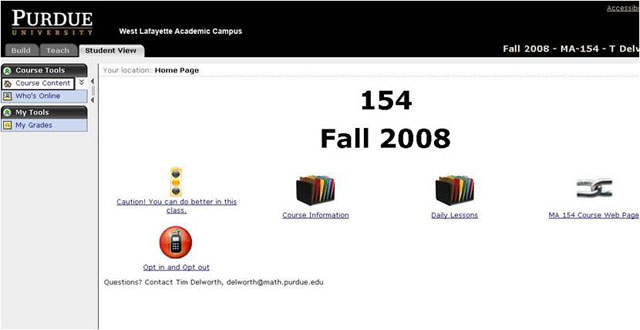
\includegraphics[scale=1]{Imagens/signals1.jpg}
  	\caption{Student dashboard (source: \cite{arnold2010signals})}
  	\label{fig:s1}
\end{figure}

\begin{figure}[htb]
	\centering
  	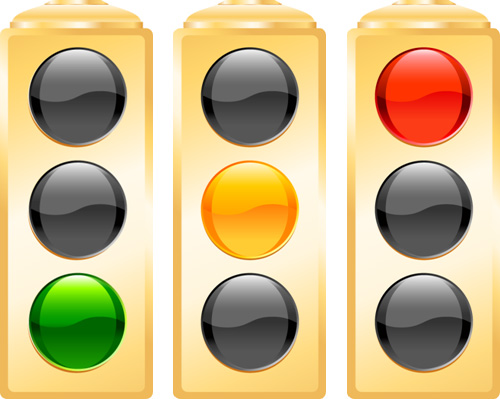
\includegraphics[scale=.3]{Imagens/signals2.jpg}
  	\caption{Traffic signals (source: \cite{arnold2010signals})}
  	\label{fig:s2}
\end{figure}

Another example of usage of these alert systems is in \cite{shi2014developing}, the authors suggests a early warning system to be used as a plugin to a learning management system\abrv{Learning Management System}{LMS}(LMS). After a student logs into the LMS (see figure \ref{fig:lms}), a dashboard with his/her current learning status is displayed (in the left side of the screen).

In addition, there is also a list of the key performance indicators, these indicators are the most important features that were calculated by the data mining engine. For each indicator, the student can see the learning history (on the right side of the screen). This learning history can also be compared with the results of the class. All of these elements can help students to monitor their performance. Thus, the system can help with the identification of at-risk students at any point in time, greatly minimizing the negative effects of poor performance.

\begin{figure}[htb]
	\centering
  	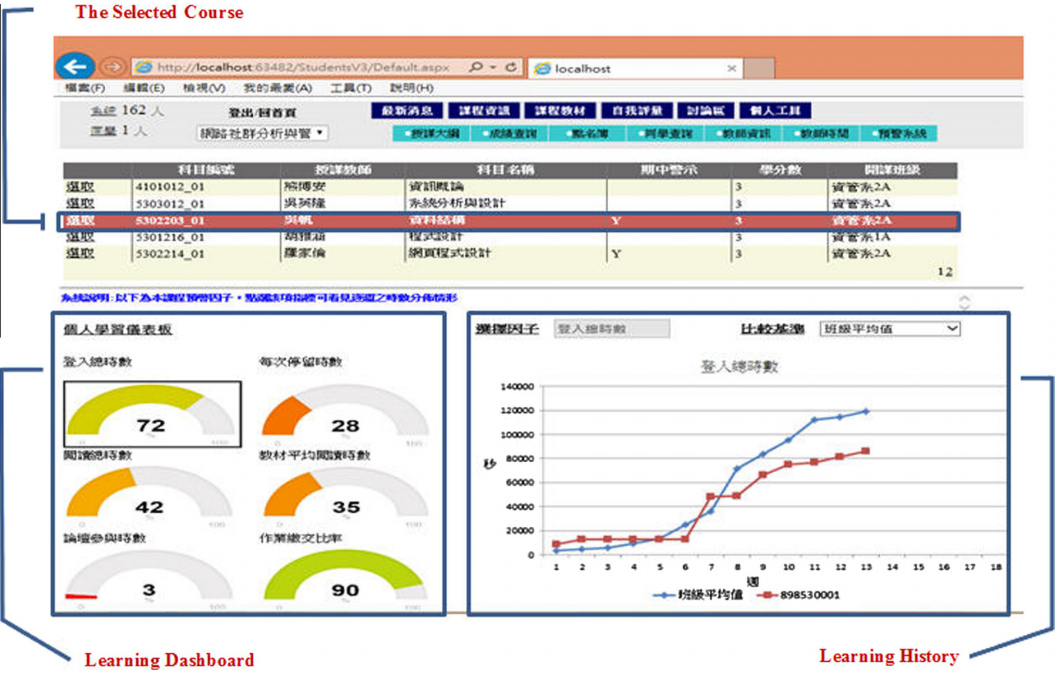
\includegraphics[scale=.5]{Imagens/lms.png}
  	\caption{Student dashboard (source: \cite{shi2014developing})}
  	\label{fig:lms}
\end{figure}

Studies show that early prediction of academic performance can be done, but the development of a generic prediction model, to be used in different courses, is a challenging task. One big reason behind this is that the different instructional conditions used in the course affect the performance of prediction models. Thus, it is important to develop and validate prediction models for each different courses \cite{akccapinar2019using}.

\section{Educational data mining (EDM)}
\label{sc:edm}

EDM\abrv{Educational Data Mining}{EDM}is a research field that applies statistics and machine learning algorithms over data generated in an educational context, to solve educational related issues. Hence, it is interested in developing methods to explore the data in an educational setting and, using these methods, to better explain students and the environment in which they learn \cite{romero2010educational}.

LA and EDM are both fields that share a common interest in data-intensive approaches to educational research to enhance the educational process. The difference is that LA focuses on the educational side and EDM focuses on the technological side. LA concentrates on data-driven decision-making and combining the technical and pedagogical dimensions of learning by putting into use known predictive models. In contrast, EDM is usually searching for new patterns in data and developing new algorithms and/or models \cite{romero2020educational}.

The four main steps of the EDM/LA process are the following \cite{sokkhey2020developing}, \cite{romero2020educational}:

\begin{enumerate}
    \item Obtain raw data
    
    In this first step, the targeted data is collected from sources as school databases or questionnaires. The are multiple types of data that can be used: educational (e.g., navigation in the virtual environment, quizzes, exercises, forum messages, etc.) administrative data (e.g., information about the school, teachers, curriculum, disciplines), demographic data (e.g., city, gender, school type, income, age, etc.), student emotions (e.g., motivation, emotional states), and so on.
    
    There are also different granularity levels (from crude to refined) or various levels of hierarchy (answer level, session-level, student level, classroom level, and school level) that can provide more or fewer data.
    
    \item Preprocessing
    
    Since the raw data can come from several different sources and have distinct formats, it is often the case that the data needs to be processed to achieve the desired format. This step also includes choosing what data to collect, making sure the data is aligned with the questions the work intends to answer. Some examples of techniques are: 
    \begin{itemize}
        \item Dealing with missing data: to handle the problem of having instances with missing values in the data set, an option is to fully discard those instances, or replace the missing values with the most frequent/average value.
        \item Discretization: transforms some continuous variable onto discrete values.
        \item Feature engineering: selecting the most important variables or creating new attributes from already existing ones.
        \item Feature scaling: some algorithms need the data to be shaped in a specific way. A few examples are:
        \begin{itemize}
            \item Normalisation: scales the features in a predetermined range (usually the 0-1 interval).
            \item Standardisation: scales the data to follow a normal distribution (usually with 0 mean and 1 standard deviation).
        \end{itemize}
    \end{itemize}
    
    \item EDM methods
    
    There is a wide range of traditional\abrv{Data Mining}{DM}DM methods that can be used in this step for solving educational problems, such as visualization, prediction, clustering and social network analysis. Table \ref{tab:edm-methods} gives more examples and details about these methods.
    
    \item Interpretation
    
    The last step brings new knowledge discovered by the DM methods to be used by teachers and students to make interventions to improve student learning performance. That is, taking action is the final goal of any learning analytics process and the outcome of follow-up actions will determine the success or failure of the analytical attempts. It is also important that the models generated in the previous step are comprehensible to be useful for those who will use the model. In this context, visualization techniques can be very useful for showing results in a way that is easier to interpret.
\end{enumerate}

An overview of the EDM/LA knowledge discovery cycle can be seen in figure \ref{fig:edm}. It shows how this method works as a cycle that aims to continuously improve the educational environment, by using the educational data to create models to be used by learners and academic authorities in an educational setting.

\begin{figure}[htb]
	\centering
  	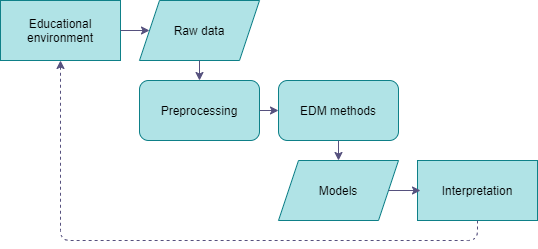
\includegraphics[scale=.7]{Imagens/edm.png}
  	\caption{EDM/LA knowledge discovery cycle (adapted from \cite{linan2015educational})}
  	\label{fig:edm}
\end{figure}

\section{Predictive analysis}

Predictive analysis is an example of a DM method that aims to estimate the value of some feature of the data set. When this value is numerical or continuous we have a regression task, when it is categorical or discrete, a classification task. Details about this method are presented in the following section \ref{sc:class}.

\subsection{Classifiers}
\label{sc:class}

Classification is one of the most popular approaches to DM. The goal is to create classification models using the training data so that results can be predicted into one of the classes of the data. The following sections were made following the works of \cite{bramer2007principles} and \cite{larose2006data}, and it displays some examples of classifiers presented in more detail.

\subsubsection{K-nearest neighbors (KNN)}

The\abrv{K-Nearest Neighbors}{KNN}KNN algorithm classifies new instances based on the \emph{closeness} to the instances that already are in the data set. For example: in a 3-NN classifier each newly added instance is classified by the votes of the 3 nearest neighbors. This voting system can be a simple best of 3 or it can weigh the votes by distance, meaning that closer neighbors will receive greater weight than the classifications of more distant ones. This classifier is used mainly when all attribute values are continuous, although it can be altered to handle categorical attributes. 
KNN is an example of a lazy learning algorithm because it uses all the data for training. Thus, it does not have a specialized training phase.

About the distance measures, there are two common ways of doing it:

\begin{itemize}
    \item Euclidean Distance: it is the default way of measuring point distance in a plane. Formally, the distance $d$ between points $a$ and $b$ is:

    \[ d(a,b) = \sqrt{\sum_{i=1}^n {(a_i - b_i)}^2} \]

    \item Manhattan Distance: it measures the distance between two data points in a grid like way. Formally, the distance $d$ between points $a$ and $b$ is:
    
    \[ d(a,b) = \sum_{i=1}^n {|a_i - b_i|} \]
\end{itemize}

Alternatively, any other method that respects the requirements of distance measures can be used. Using the notation $d(X,Y)$ to stand for the distance between points $X$ and $Y$, these conditions are:

\begin{enumerate}
    \item $d(A,A) = 0$, meaning that the distance of any point A to itself is zero.
    \item $d(A,B) = d(B,A)$ is the symmetry condition. In other words, the distance from $A$ to $B$ is the same as from $B$ to $A$.
    \item $d(A,B) \le d(A,C) + d(C,B)$ is the triangle inequality. It captures the idea that 'the shortest distance between any two points is a straight line'.
\end{enumerate}

It is important to notice that these ways of measuring distance can work badly if the data is not in the same range of values. This happens because large values will weigh more than small ones. So, before running the classifier it is critical to normalize the features.

In real problems, a common value for K is the square root of the data set size. Also, an odd value for K is desired to avoid confusion between two classes. If it is chosen K values that are low, the results should be less biased but with higher variance, but when the K values are high, the results should have less variance and higher bias. This is what is called the \emph{bias–variance dilemma}. In other words, it is the conflict in trying to minimize those two types of error simultaneously.

In summary, the algorithm for the KNN classifier is:

\begin{algorithm}[H]
Step 1 - find the k \emph{closest} instances to the new instance. \\
Step 2 - use a voting system to choose a class from these k instances as the result.
\caption{KNN}
\end{algorithm}

\subsubsection{Naive Bayes}

Naive Bayes is a set of classifiers that uses concepts of probability theory to find the most likely possible classification for each new instance. The algorithm combines prior probability and conditional probabilities into a formula that can calculate the probability of each class. Prior probability is defined as the probability of an event before new data is collected, and conditional probability is the probability of an event occurring, given that another event happened. These concepts are the basis for the Bayes' theorem, formally defined as:

\[ P(A|B) = \frac{P(B|A)P(A)}{P(B)} \]

Where A and B are events, and P(X) is the probability of X. P(A) is called \emph{priori} or prior probability of A, and P(A|B) is a \emph{posteriori} probability of B, meaning the probability of a event after some evidence is seen.

Formally, a Bayes classifiers' definition is: given a set of $n$ classes $c_1$, $c_2$, ..., $c_n$, which have prior probabilities $P(c_1)$, $P(c_2)$, ..., $P(c_n)$, respectively, and m features $a_1$, $a_2$, ..., $a_m$, and given a new instance with features' values $v_1$, $v_2$, ..., $v_m$, the probability of each class will be proportional to:

\[ P(c_i) \times \prod_{j=1}^m P(a_m=v_m | class = c_i) \]

Finally, the class for each new instance will be stated as the class with higher probability.

The formula above assumes that all attributes are independent (hence the \emph{naive} in the methods' name). Another restriction is that this formula works only with categorical features. To overcome this, a specific type of Bayes classifier must be used: Gaussian Naive Bayes, where continuous values of each feature are assumed to be distributed according to a Gaussian distribution. Even with all of these assumptions, the Naive Bayes method often gives good results in real problems.

In short, the algorithm for the Naive Bayes classifier is:

\begin{algorithm}[H]
Step 1 - calculate the classes' prior probabilities. \\
Step 2 - calculate the conditional probabilities of the new instances' attributes for each class. \\
Step 3 - the result will be the class with higher probability.
\caption{Naive Bayes}
\end{algorithm}

\subsubsection{Random Forest}

Random Forest is an example of ensemble classification. The idea behind this concept is to learn not just from one classifier but a set of classifiers, called an ensemble of classifiers so that their predictions for the class of unseen instances are combined in some way. In random forests, the ensemble is a set of decision trees, so it is called a homogeneous ensemble as all classifiers are of the same kind.

There are a few ways in which an ensemble can be created, for example:

\begin{itemize}
    \item N trees made using the same tree generation algorithm, but with different parameter settings, all using the same training data.
    \item N trees made using the same tree generation algorithm, all with different training data and either with the same or with different parameter settings.
    \item N trees made using a variety of distinct tree generation algorithms, either with the same or with different training data.
    \item N trees made using a different subset of the features for each one.
\end{itemize}

It can be noticed that this process is computationally more expensive more than building a single tree, but it is wished that the ensemble will collectively have higher accuracy than any one of the individual classifiers. In section \ref{sc:training} it is described the standard methodology for evaluating the performance of a classifier. For an ensemble classifier, the method requires an additional data set called a validation data set associated with each classifier. This procedure works as follow:

\begin{enumerate}
    \item Divide the data set into a test set and the rest.
    \item For each classifier:
        \begin{enumerate}
        \item Divide the remaining data from step (1) into training data and validation data in some sort of way.
        \item Create the classifier using the training data.
        \item Estimate the performance by running the classifier against the validation data set.
    \end{enumerate}
    \item Find the best classifiers by using those with greater accuracy than some threshold or choose the best N classifiers.
    \item Use the ensemble to classify each of the samples in the test set selected at step (1). This result will be an estimate of the performance of the ensemble on unseen data.
\end{enumerate}

An approach to implement the step (2)(a) is called bagging, and it works the following way:

\begin{itemize}
    \item Randomly select N instances from the remaining data, one-by-one, at each stage selecting from the full set of instances (so it is sampling with replacement). Doing this will inevitably led to a training set with instances that appear more than once, perhaps several times, and others will not appear at all.
    \item The instances left unselected by this process will form a validation set.
\end{itemize}

At step (4) it is common to use each of the classifiers independently and then to combine their votes for the correct classification, this approach is called majority voting.

In conclusion, the algorithm for the Random Forest classifier is:

\begin{algorithm}[H]
Step 1 - Generate N trees for a given data set. \\
Step 2 - For a new unseen sample X: \\
Step 2 (a) - Calculate the predicted classification of X for each of the N classifiers. \\
Step 2 (b) - Select the class using some voting system.
\caption{Random Forest}
\end{algorithm}

\subsubsection{Logistic Regression}

Logistic Regression is a method that describes the relationship between a categorical result variable and a set of predictor variables. It is in many ways similar to linear regression with the main difference that the result is binary rather than continuous. Linear Regression assumes a relationship between predictor and response variables that is linear. In this case, the least-squares regression line is used as the method to find the line that best fits the data. In contrast, the Logistic Regression assumes that the relationship between the predictor and the response is nonlinear. In this case, the model is represented by an S-shaped (sigmoidal) curve (see figure \ref{fig:sig}).

\begin{figure}[htb]
	\centering
  	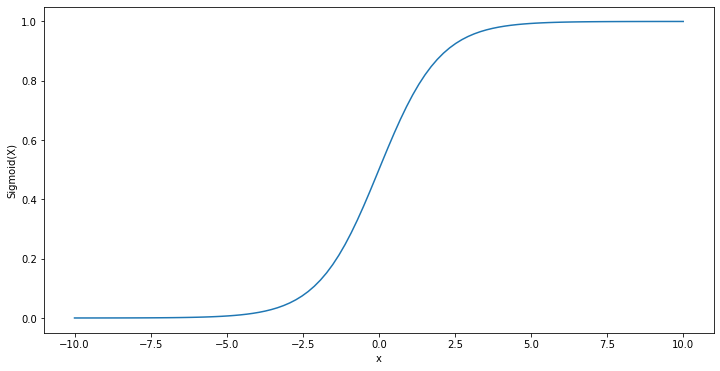
\includegraphics[scale=.5]{Imagens/sigmoid.png}
  	\caption{Logistic Regression curve}
  	\label{fig:sig}
\end{figure}

In Logistic Regression the best fitting line is estimated using the maximum likelihood method, which finds the coefficients for which the likelihood of observing the data is maximized. The maximum likelihood estimators are commonly solved by iterative methods such as iterative weighted least squares (see \cite{nelder1972generalized}).

The Logistic Regression method offers some interpretations that are easy to understand. The y axis can be interpreted as the probability $\pi(x)$ that some instance belongs to a default class. This default class is what is assigned to $Y=1$. For example, if the problem is to classify if a picture has a cat, the $Y=1$ could mean that the picture has a cat, while $Y=0$ that the picture has no cat. Formally, the probability that an input (X) belongs to a default class (Y=1) is:

\[ P(X) = P(Y=1|X) \]

The logistic regression function, where $\beta_0$ and $\beta_1$ are the coefficients, is:

\[ \pi(x) = \frac{e^{\beta_0+\beta_1x}}{1+e^{\beta_0+\beta_1x}} \]

Another important equation is the \emph{logit} transformation:

\[ g(x) = ln\frac{\pi(x)}{1-\pi(x)} = \beta_0+\beta_1x \]

This ratio in the middle is called the \emph{odds} of the default class. Odds are an important concept that can be defined as the probability that an event occurs divided by the probability that the event does not occur. When odds > 1 the event is more likely to occur, and when odds < 1 the event is more likely to not occur.

The logit has several attractive properties of the linear regression model, such as linearity, continuity, and range from negative to positive infinity. The coefficient $\beta_0$ (intercept) can be interpreted as assuming a value of 0 for all the predictors in the model. Further, the coefficient $\beta_1$ (slope) can be interpreted as the change in the response variable for every unit increase in the predictor. In short:

\[ \beta_1 = g(x+1) - g(x) \]

In summary, the algorithm for the Logistic Regression classifier is:

\begin{algorithm}[H]
Step 1 - Use a maximum likelihood method to find the logistic regression function's coefficients. \\
Step 2 - Plug in the values of the new instances' attributes. \\
Step 3 - The result class will be the default class (Y=1) if the probability is closer to 1. Otherwise, it will be the other class (Y=0). 
\caption{Logistic Regression}
\end{algorithm}

\section{Model training and performance evaluation}
\label{sc:training}

In the process of creating models, there are two distinct phases: building and evaluating the models. The data set for each of these phases is a partition of the original data set. This way, there are at least two sets: the training set, for building the model; and the testing set, for the evaluation. In the building phase, the classifiers' algorithms aim to create a function that best maps the data attributes to data classes, while the testing phase looks to evaluate the predictive aspect of the model to new data not previously seen \cite{cechinel2020mineraccao}.

The following section \ref{sc:dp} shows the common ways of partitioning the data set, section \ref{sc:ht} presents a method used to improve the classifiers' performance, and, finally, section \ref{sc:pm} shows ways to evaluate the performance of the DM algorithms.

\subsection{Data partitioning}
\label{sc:dp}

There are different ways that the data set can be partitioned into training and testing sets. In some cases, it already exists some natural way of dividing the data set. For example, if we wish to build a model to classify students by either pass or fail in a class, given that this class was offered in distinct semesters, we could test the data with some semester $A$ and train the data with the remaining semesters. When there is not an obvious way to divide the data, the alternative is to use some data partitioning technique. Holdout and k-fold cross-validation are the two main methods to partition the data.

\subsubsection{Holdout}

The holdout method randomly divides the data into two sets that does not overlap. It is common to use 75\% of data for training and 25\% for testing, but this is not a universal rule. This method is usually used when the data set has a large amount of samples.

\subsubsection{K-fold cross-validation}

The k-fold cross-validation method is a type of validation that splits the data set into k folds and uses k-1 folds for training and the remaining fold for testing. This procedure is repeated k times so that each fold has been used for testing exactly once. Finally, the performance metrics are calculated based on the average performance of those repetitions. A common number of folds used in real applications is 10, a so-called 10-fold. It is usually used when the data set has a limited amount of samples.

\subsection{Hyperparameter tuning}
\label{sc:ht}

The ML algorithms often have parameters that can be adjusted to develop the most optimal model. These are called "hyperparameters". A popular technique used in hyperparameter selection is grid search. In this approach, the parameters of the classifiers are exhaustively searched through a manually specified subset of the possible values to those parameters.

\subsection{Performance metrics}
\label{sc:pm}

Considering the characteristics of each data set and which model was used, different metrics can be used for model evaluation. This section presents the most common metrics for the evaluation of classifiers.

\subsubsection{Confusion matrix}
When working on a classification problem it is common to divide the data set into two classes. In this situation, the predictive performance of the model can be described in a 2x2 matrix that is called a binary confusion matrix. This matrix has labels for the real and observed classes of the data. Hence, there are four possible combinations: True positive (TP) and true negative (TN), relating to the correct answers; false positive (FP) and false negative (FN), relating to the incorrect answers, as can be seen in the table \ref{tab:cm}.

\begin{table}[htb]
\centering
\begin{tabular}{|c|c|c|c|}
\hline
\multirow{2}{*}{} & \multirow{2}{*}{} & \multicolumn{2}{c|}{Actual value} \\ \cline{3-4} 
 &  & True & False \\ \hline
\multirow{2}{*}{\begin{tabular}[c]{@{}c@{}}Model\\ prediction\end{tabular}} & True & \begin{tabular}[c]{@{}c@{}}True Positive\\ (TP)\end{tabular} & \begin{tabular}[c]{@{}c@{}}False Positive\\ (FP)\end{tabular} \\ \cline{2-4} 
 & False & \begin{tabular}[c]{@{}c@{}}False Negative\\ (FN)\end{tabular} & \begin{tabular}[c]{@{}c@{}}True Negative\\ (TN)\end{tabular} \\ \hline
\end{tabular}
\caption{Binary confusion matrix}
\label{tab:cm}
\end{table}

\subsubsection{Accuracy}

Accuracy is often used as a performance metric of classifiers. It measures the rate of correctly classified instances. Formally:

\[ Accuracy = \frac{number\ of\ correct\ predictions}{total\ number\ of\ predictions} \]

When dealing with a binary classification problem, it can also be defined as:

\[ Accuracy = \frac{TP+TN}{TP+TN+FP+FN} \]

\subsubsection{True Positive Rate (TPR)}

The\abrv{True Positive Rate}{TPR}TPR is the ratio between the correctly classified as true instances and all true instances. This metric can also be called as Recall or Sensitivity. Formally:

\[ TPR = \frac{TP}{TP+FN} \]

\subsubsection{True Negative Rate (TNR)}

The\abrv{True Negative Rate}{TNR}TNR is the ratio between the correctly classified as false instances and all false instances. This metric is also called Precision or Specificity. Formally:

\[ TNR = \frac{TN}{TN+FP} \]

\subsubsection{F-Measure}

The F-Measure combines TPR and TNR by calculating the harmonic average of them. This is done to avoid biased comments in the evaluation of models by using TPR or TNR separately. Formally defined as: 

\[ F\mbox{-}Measure = \frac{2TP}{2TP+FP+FN} \]

\begin{table}[htb]
\centering
\begin{tabular}{lll} \hline
\textbf{Method} & \textbf{Goal/description} & \textbf{Applications} \\ \hline
Causal mining & \begin{tabular}[c]{@{}l@{}}To find causal relationship or\\ patterns in data.\end{tabular} & \begin{tabular}[c]{@{}l@{}}Finding what attributes of\\ students' behavior cause\\ learning, academic failure,\\ and so on.\end{tabular} \\ \hline
Visualization & To show a graphical view of data. & \begin{tabular}[c]{@{}l@{}}Data visualizations tools\\ that help inform results of\\ EDM/LA research\\ to educators.\end{tabular} \\ \hline
Prediction & \begin{tabular}[c]{@{}l@{}}To infer a target variable\\ from some combination\\ of other variables.\\ Classification and regression\\ are examples of\\ prediction methods.\end{tabular} & \begin{tabular}[c]{@{}l@{}}Predicting student\\ performances.\end{tabular} \\ \hline
Clustering & To group similar students. & \begin{tabular}[c]{@{}l@{}}Grouping similar\\ materials or students\\ based on their \\ learning patterns.\end{tabular} \\ \hline
\begin{tabular}[c]{@{}l@{}}Social network\\ analysis\end{tabular} & \begin{tabular}[c]{@{}l@{}}To analyze the social relationships\\ between individuals in a network.\end{tabular} & \begin{tabular}[c]{@{}l@{}}Analysis of the structure\\ and relations\\ in collaborative tasks.\end{tabular} \\ \hline
Recommendation & \begin{tabular}[c]{@{}l@{}}To calculate the rating\\ or preference\\ a user would give to an item.\end{tabular} & \begin{tabular}[c]{@{}l@{}}To make recommendations\\ to students related to their\\ activities, tasks, links to visit,\\ problems to solve\\ or courses to take, and so on.\end{tabular} \\ \hline
Outlier detection & \begin{tabular}[c]{@{}l@{}}To identify significantly\\ different individuals.\end{tabular} & \begin{tabular}[c]{@{}l@{}}Detection of students with\\ learning difficulties.\end{tabular} \\ \hline
Statistics & \begin{tabular}[c]{@{}l@{}}To calculate descriptive and\\ inferential statistics.\end{tabular} & Interpreting educational data. \\ \hline
Text mining & \begin{tabular}[c]{@{}l@{}}To extract information\\ from text.\end{tabular} & \begin{tabular}[c]{@{}l@{}}Analyzing the contents\\ of documents, chats,\\ forums and web pages.\end{tabular} \\ \hline
\end{tabular}
\caption{Popular EDM/LA methods (adapted from \cite{romero2020educational})}
\label{tab:edm-methods}
\end{table}

	\chapter{Methodology}
\label{ch:Methodology}

This work is applied research because it is designed to build a tool to solve an existing issue in the context of a real organization. The research will use a method for data analysis already established in the context of EDM problems, as it was described in section \ref{sc:edm}, where data will be collected, then DM algorithms will be applied to that data and, finally, a comparative analysis between those algorithms will be made. Because of this approach, it can be said that the research uses quantitative methods \cite{gomes2019classificaccao}.

Further, this research follows the procedure defined by Design Science Research\abrv{Design Science Research}{DSR}(DSR). DSR is commonly used when the researcher is interested in (1) solve a practical problem in a specific context through the development of an artifact, which is anything built to reach an objective; and (2) produce new knowledge. DSR is based on two cycles (1) design cycle, which aims to create an artifact, evaluate and refine the project; and (2) knowledge cycle, which aims to elaborate theoretical suppositions related to human behavior, that has phases such as validation, execution, analysis, and research contribution \cite{pimentel2019design}.

Following the objectives of DSR, this work aims to build a web system as a new software artifact and intends to create new knowledge about this research topic. Figure \ref{fig:dsr} presents the two cycles of DSR and how it is used by this research. It can be seen that the evaluation is based on three aspects: (1) if the artifact meets the requirements, (2) if the problem was successfully solved, and (3) if the theoretical conjectures seem valid.

\begin{figure}[htb]
	\centering
  	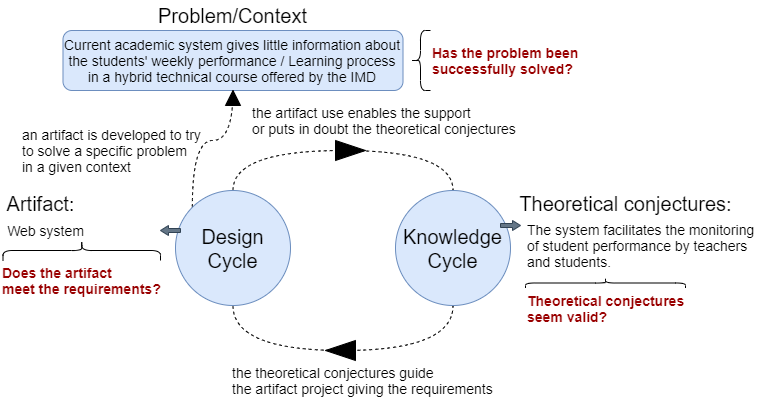
\includegraphics[scale=.55]{Imagens/dsr.png}
  	\caption{DSR process (adapted from \cite{pimentel2019design})}
  	\label{fig:dsr}
\end{figure}

The central objective of this research is to develop a web system for student performance prediction that helps with the learning process that the students from the IMD's IT technical course go through. This system will use DM techniques with the educational data provided by the Sistema Integrado de Gestão de Atividades Acadêmicas\abrv{Sistema Integrado de Gestão de Atividades Acadêmicas}{SIGAA}(SIGAA), which is the system used at IMD to manage the academic environment.

The main stakeholders associated with this research are the teachers and students of the IMD. It is hoped that the proposed web system can help teachers detect students that may require additional support, and give the students another way of monitoring their performance, thus, enhancing their academic experience.

The following sections present details about the data set, tools needed and a list of the project activities.

\section{Data set}

The data was requested to Superintendência de Tecnologia da Informação (STI), the university sector responsible for the SIGAA system, in early April 2021. Soon after, it was received a single report file in a comma-separated values file with all the required data. The structure of the data set is presented in appendix \ref{ch:Dataset}.

Before requesting the data a few project decisions were made, based on previous knowledge about the IMD's IT technical course structure: (1) work only with data from classes in the first semester of the course. This choice was made given how much more data is available relative to classes from the following semesters. (2) Use only data from the most recent curriculum, for the same reason as the previous decision. In addition, it was not requested any sensitive information about the students. This was done to preserve learners' information because of privacy regulations, and also because to achieve the goals of this research it is sufficient to use only data about scores and attendance of students.

The full data set has a total of 127 features and 6316 samples. The data ranges between years 2015 and 2020 and contains the scores and attendance of the students in all classes (6 in total), all weeks (up to 20 weeks), scores by different tasks (4 distinct types of tasks), and the final result in the first semester of the course. Details about the distribution of the samples through the years are shown in table \ref{tab:sbys}.

\begin{table}[htb]
\centering
\begin{tabular}{cc} \hline
\textbf{Semester} & \textbf{Number of samples} \\ \hline
2015.1 & 1351 \\
2016.1 & 1160 \\
2017.1 & 1076 \\
2017.2 & 697 \\
2018.1 & 639 \\
2019.1 & 634 \\
2020.1 & 759 \\ \hline
\end{tabular}
\caption{Amount of samples in the data set by semester}
\label{tab:sbys}
\end{table}

\section{Tools}

The data analysis step of the project was developed using Python\footnote[1]{\hspace{1mm}\url{https://www.python.org}} programming language and the Google Colaboratory\footnote[2]{\hspace{1mm}\url{https://colab.research.google.com}} environment. The Python language was chosen given the easiness of use and broad ecosystem available to solve DM problems. The libraries used are the following: pandas\footnote[3]{\hspace{1mm}\url{https://pandas.pydata.org}} and NumPy\footnote[4]{\hspace{1mm}\url{https://numpy.org}} (for data analysis and scientific computing), Matplotlib\footnote[5]{\hspace{1mm}\url{https://matplotlib.org}} and Seaborn\footnote[6]{\hspace{1mm}\url{https://seaborn.pydata.org}} (for data visualization) and scikit-learn\footnote[7]{\hspace{1mm}\url{https://scikit-learn.org/stable/index.html}} (for the machine learning algorithms).

The web system was also developed using Python. The server was built using Flask\footnote[8]{\hspace{1mm}\url{https://flask.palletsprojects.com/en/2.0.x/}}, a micro web application framework, and Jinja\footnote[9]{\hspace{1mm}\url{https://www.palletsprojects.com/p/jinja/}} as the template engine. The libraries used are: Flask-RESTful\footnote[10]{\hspace{1mm}\url{https://flask-restful.readthedocs.io/en/latest/}} (for building the mock\abrv{Application Programming Interface}{API}API server), requests\footnote[11]{\hspace{1mm}\url{https://docs.python-requests.org/en/master/}} (for queries to the API), Bootstrap-Flask\footnote[12]{\hspace{1mm}\url{https://bootstrap-flask.readthedocs.io/en/stable/index.html}} (for the templates of the web system's pages), and joblib\footnote[13]{\hspace{1mm}\url{https://joblib.readthedocs.io/en/latest/}} (to manipulate the DM models' files).

\section{Project activities}

Based on the EDM process, this research was developed according to the following tasks:

\begin{enumerate}
    \item Define the problem this work aims to solve, after an analysis of the current state of the virtual learning environment used by the students of the IMD.
    \item Obtain the raw educational data that will be used in the research.
    \item Apply preprocessing techniques in that data to reduce complexity and prepare the data to be effectively used by the DM algorithms.
    \item Research the DM algorithms that are commonly used in predictive systems.
    \item Analysis of those algorithms aiming to find the model with the best results for the given data.
    \item Develop a web system prototype to be used by teachers and students for the visualization of the likelihood the student has to pass the course.
\end{enumerate}
	
	\chapter{Experiments and results}
\label{ch:Experiments}

This chapter presents the results attained by applying the EDM process to the educational data set of the IMD's students and the proposed web application that uses the selected models. Before showing the results it is important to understand how the academic performance is done in the IMD's IT course: the students' final grade is a combination of four distinct tasks. Two of these tasks are done at the end of the course and combined weighs 65\% of the final grade. The other two tasks are done and graded weekly, combining 35\% of the final grade. The analysis done in this research uses only those weekly grades.

To give an overview of the data set, descriptive statistics are shown in table \ref{tab:da}, and a histogram of the students' final score, grouped by pass (True) or fail (False), is shown in figure \ref{fig:mm}. It can be noticed that it exists a balance in the data set between classes Pass and Fail. This is important because some of the classifiers' algorithms could perform poorly if the data set is imbalanced. Grades have a peak of occurrences around 5, which is the minimum grade for passing, and another peak around 0, most likely indicating those students who gave up the course.

\begin{table}[ht]
\centering
\begin{tabular}{ccc} \hline
\textbf{Final result} & \textbf{Number of students} & \textbf{Percentage of students} \\ \hline
Pass                  & 3427                        & 56.47\%                         \\
Fail                  & 2642                        & 43.53\%                         \\ \hline
\end{tabular}   
\caption{Final situation of students in classes}
\label{tab:da}
\end{table}

\begin{figure}[htb]
	\centering
  	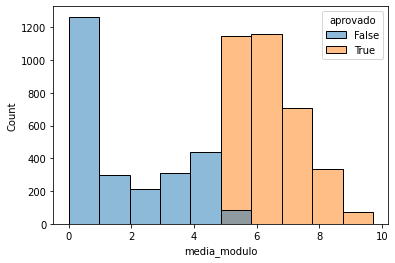
\includegraphics[scale=.5]{Resultados/mm.png}
  	\caption{Students' final score}
  	\label{fig:mm}
\end{figure}

\section{Data preprocessing}
The first action in the preprocessing stage was to select the most relevant features. The original data set had a total of 127 features, but some of these features are either a combination of other attributes or are scores determined only at the end of the course. As the focus of this research is only on the weekly grades and attendance data, it was decided to reduce the data set.

In addition, features of weeks 19 and 20 (the last two weeks in the data set) were dropped due to the amount of missing data, as seen in table \ref{tab:featmiss}. Besides that, two features were replaced to represent the classes of the problem, either for the binary or 3-class problem. One of these attributes was the final grade that was changed from a continuous variable to a nominal variable with three distinct classes. The other one was the final result class that was changed from a nominal variable (with distinct classes to indicate if the student passed or failed) to a binary.

\begin{table}[ht]
\centering
\begin{tabular}{cc} \hline
\textbf{Feature} & \textbf{Percentage of missing values} \\ \hline
pp17 & 2.58\% \\
pv17 & 2.37\% \\
f17 & 2.58\% \\
pp18 & 8.76\% \\
pv18 & 8.55\% \\
f18 & 8.76\% \\
pp19 & 39.36\% \\
pv19 & 39.14\% \\
f19 & 39.36\% \\
pp20 & 77.73\% \\
pv20 & 77.73\% \\
f20 & 77.73\% \\ \hline
\end{tabular}
\caption{Percentage of missing values of last weeks' features}
\label{tab:featmiss}
\end{table}

To sum up, after the preprocessing, the reduced data set, used by the classifiers, had a total of 56 features that can be seen in detail in table \ref{tab:Dataset2}.

The next action was dealing with missing data. In this step data from students that canceled the course was removed. Most of the students' dropping out happened in the 2020.1 semester, an atypical semester that, due to the COVID-19 pandemic, was not done in the usual hybrid format. The semester started as usual but by the 4th-week classes were stopped returning 12 weeks later with only online classes. The students were given the choice to continue in this new format or to drop out of the course. This action implied losing 247 of the 6316 samples (3.91\% of the data set). Data is shown in detail in table \ref{tab:dropouts}.

\begin{table}[ht]
\centering
\begin{tabular}{cccc}
\hline
\textbf{Semester} & \begin{tabular}[c]{@{}c@{}}\textbf{Number of}\\ \textbf{students}\end{tabular} & \begin{tabular}[c]{@{}c@{}}\textbf{Number of}\\ \textbf{dropped out}\\ \textbf{students}\end{tabular} & \textbf{Dropout rate} \\ \hline
2015.1 & 1351 & 0 & 0.00\% \\ 
2016.1 & 1160 & 0 & 0.00\% \\ 
2017.1 & 1076 & 0 & 0.00\% \\ 
2017.2 & 697 & 0 & 0.00\% \\ 
2018.1 & 639 & 0 & 0.00\% \\ 
2019.1 & 634 & 7 & 1.10\% \\ 
2020.1 & 759 & 240 & 31.62\% \\ \hline
\end{tabular}
\caption{Students' dropout rate}
\label{tab:dropouts}
\end{table}

The remaining missing values were updated with the mean value for the feature, as this is a usual way of dealing with missing data. Finally, the last action was to scale the data so that all features share the same range. This was done because some of the algorithms used need it to work properly. So, all numeric features were scaled to the [0, 1] interval.

\section{Data analysis}

The problem of predicting students' end-of-term results is an example of a classification problem. In this work, the results for a binary problem (final result can be either 'Pass' or 'Fail') and also for a 3-class problem (final result can be either 'High risk', 'Middle risk' or 'No risk') were calculated.

In related works \cite{akccapinar2019using} \cite{khalil2015learning}, numerous algorithms are cited as able to solve this kind of problem. So, in this work, the following algorithms were selected: Naive Bayes, KNN, Random Forest, and Logistic Regression. The performance of these selected algorithms was initially compared based on accuracy.

For the 3-class problem, the final students' grades were grouped in 3 classes determined by applying the K-Means algorithm, a clustering algorithm that partitions a set of values into k sets, to the students' final grade. The centroids of the three classes are 0.78, 4.92, and 7.06. Details about the classes' balance using those groups are shown in table \ref{tab:3c}.

\begin{table}[htb]
\centering
\begin{tabular}{ccc} \hline
\textbf{Class} & \textbf{Number of students} & \textbf{Percentage of students} \\ \hline
High risk                & 2202                        & 36.43\%               \\
Middle risk              & 1760                        & 29.12\%               \\
No risk                  & 2082                        & 34.45\%               \\ \hline
\end{tabular}
\caption{3-class frequency distribution}
\label{tab:3c}
\end{table}

The performance results were obtained using a 4-fold cross validation method in all analyses. Finally, before obtaining the scores of the classifiers performance, a grid search was done to optimize the parameters of the algorithms. The final parameters, used in all analyses, are shown in table \ref{tab:param}. To clarify, the $p=1$ parameter in the KNN classifier indicates that the distance measure is the Manhattan distance.

\begin{table}[ht]
\centering
\begin{tabular}{cc}
\hline
\textbf{Classifier}                                & \textbf{Parameters}                                                                                  \\ \hline
KNN & \begin{tabular}[c]{@{}l@{}}weights='distance'\\ p=1\\ n\_neighbors=10\end{tabular}                   \\ \hline
Logistic regression                                & \begin{tabular}[c]{@{}l@{}}max\_iter=500\\ solver='newton-cg'\end{tabular}                           \\ \hline
Naive Bayes                                        &                                                                                                      \\ \hline
Random forest                                      & \begin{tabular}[c]{@{}l@{}}max\_features=None\\ criterion='entropy'\\ n\_estimators=200\end{tabular} \\ \hline
\end{tabular}
\caption{Classifiers' parameters}
\label{tab:param}
\end{table}

\subsection{Results}
The first results summarize the classifiers' accuracy using all data up to a given week, in other words, all available data of grades and attendance for any given week is used to train and test the model. These results are exhibited in figures \ref{fig:ab} and \ref{fig:a3c}, and it shows that the results were similar with a slight advantage to the Logistic Regression model that obtained better results in early weeks. For this reason, this classifier was chosen to further analysis.

The results of the Logistic Regression classifier are shown in more detail in table \ref{tab:lr}, with multiple performance metrics. The 3-class results are the mean of each metric for each label. These results show that in both binary and 3-class problems the F-Measure is even better than accuracy and that in the binary problem the recall always yields the best results between the different metrics. The high recall measures could indicate that the models are good at minimizing false negatives.

The second results were obtained by using the Logistic Regression classifier again but with different subsets of attributes from the reduced data set. This was done to see the difference in results in comparison to using the full set of features. The subsets of attributes with its description are detailed in table \ref{tab:fd} and the results are shown in figures \ref{fig:lrb} and \ref{fig:lr3c}. These results indicate that the model using all grades' features and leaving the attendance out is close in performance to the model using the full set of features. For this reason the final chosen model was the Logistic Regression classifier using only the grades' features.

\begin{table}[htb]
\centering
\begin{tabular}{cc} \hline
\textbf{Set of features} & \textbf{Description} \\ \hline
pp+pv+f & Full set of features. \\ \hline
pp+pv & Combines all grades' features. \\ \hline
pp & Features of grades' score in activities made in the classroom. \\ \hline
pv & \begin{tabular}[c]{@{}c@{}}Features of grades' score in activities \\ made in the virtual learning environment.\end{tabular} \\ \hline
f & Features about attendance. \\ \hline
\end{tabular}
\caption{Description of the features' set}
\label{tab:fd}
\end{table}

After these results, because of the better performance, the binary Logistic Regression classifier was chosen to be integrated into the web application. The models were built dropping the scaling in features to the [0, 1] interval, this way, all attributes stayed in the [0, 10] interval. The full set of models is shown in appendix \ref{ch:Models}. The default class (Y=1) indicates that the student is likely to pass the course.

Given these models, some interpretations could be made, such as the current week's coefficients are usually the greatest and that between type 1 grade (pp), activities made in the classroom, and type 2 grade (pv), activities in the virtual learning environment, the latter usually weigh more. Thus, the type 2 grade could have more influence on the students' chances of passing. Also, it is possible to plot the Logistic Regression function fixing all but one feature, this way it can be seen what impact one specific grade has in the students' chances, according to the model.

For example, using the week 4 model and the median values of the attributes of previous weeks the figure \ref{fig:w4m} plot can be made. This graph indicates that if the student receives a 3.5 or more in type 1 grade (pp) chances are in his or her favor, same for type 2 grade (pv) starting at 6.55.

\begin{figure}[htb]
	\centering
  	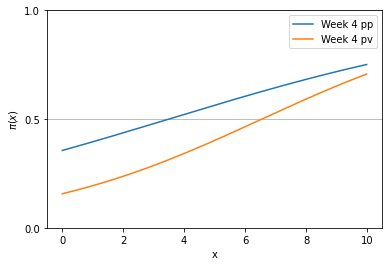
\includegraphics[scale=.5]{Resultados/week4models.png}
  	\caption{Logistic Regression function of week 4 model}
  	\label{fig:w4m}
\end{figure}

\section{Web system design}
The proposed web application's purpose is to act as an early warning tool to help students and teachers visualize current academic performance and estimated chances of success. Thus, three main components are necessary to the development of the application: (1) a source of the educational data, (2) the models that predict academic performance, and (3) a server to integrate the two previous components and exhibit the results to the users.

In summary, the server is structured as shown in figure \ref{fig:server}.

\begin{figure}[htb]
	\centering
  	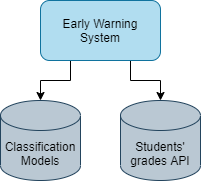
\includegraphics[scale=.7]{Imagens/server-model.png}
  	\textsf{\caption{Web server architecture}
  	\label{fig:server}}
\end{figure}

Firstly, the source of the data should be the official University's API\footnote[1]{\hspace{1mm}University's API services available in: \url{https://api.ufrn.br/}} but as the required data of students' grades were not available at the time of this research, a mock API server was built to replace the official API in the main server. The mocked server simulates only three services: get data from the logged-in user, the users' classes, and the users' grades in a class.

Secondly, the Logistic Regression binary models, from week 1 to 18, were exported and added to the main server. These models are small files that were fast to build and are fast to make predictions. This was expected as the Logistic Regression models are easy to represent as they are essentially storing the intercept and coefficients of the models.

Finally, the main server was built. The system login page should use the unified authentication of the University's API applications (see figure \ref{fig:login}). After the user is logged on, the server verifies the class that the user is enrolled then queries the API to obtain either the students' grades or the teacher's class grades, the next stage is to apply the models to classify each student in each week as either likely or not to pass the course, to subsequently exhibit this information in a simple dashboard.

The student dashboard shows cards from all weeks of the course, the scores, and performance indicators in each week (see figure \ref{fig:webs}) that are either green or red. Green indicates that the student is likely to succeed, otherwise, it is red. The teacher dashboard will show a table crossing data from students and weeks of the course (see figure \ref{fig:webp}) and indicators. These indicators are calculated the same way as it is for the student.

\begin{figure}[!htb]
   \begin{minipage}{0.48\textwidth}
     \centering
     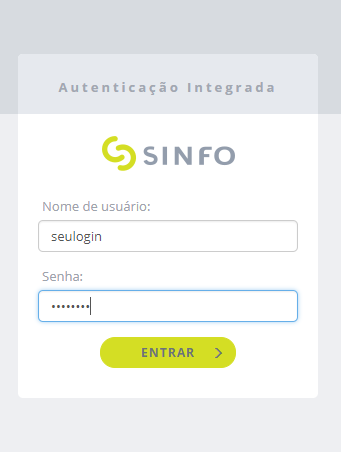
\includegraphics[width=.9\linewidth]{Imagens/login.png}
     \caption{Login page}\label{fig:login}
   \end{minipage}\hfill
   \begin{minipage}{0.48\textwidth}
     \centering
     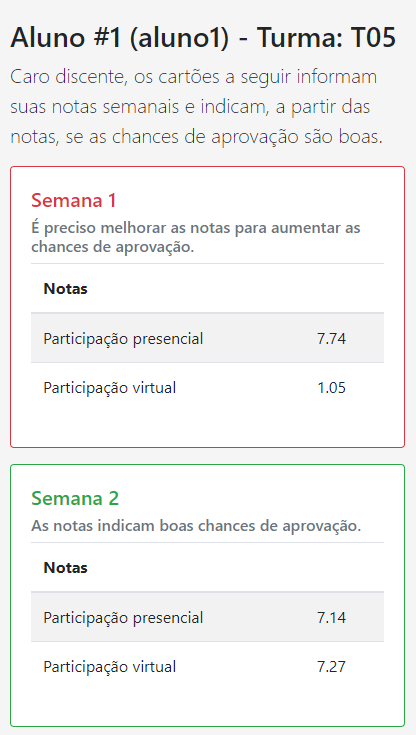
\includegraphics[width=.8\linewidth]{Resultados/web-student.png}
     \caption{Student dashboard}\label{fig:webs}
   \end{minipage}
\end{figure}

\begin{figure}[htb]
	\centering
  	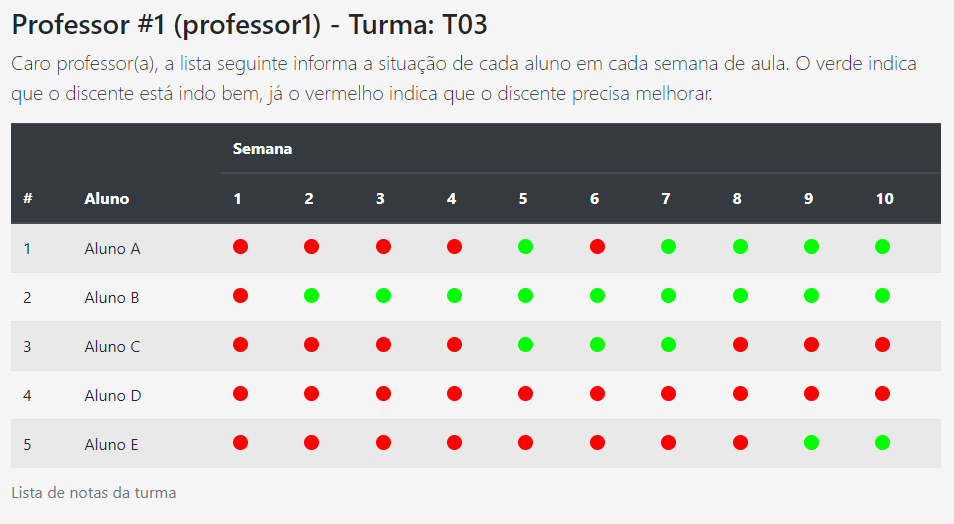
\includegraphics[scale=.6]{Resultados/web-teacher.png}
  	\textsf{\caption{Teacher dashboard}
  	\label{fig:webp}}
\end{figure}


	
	\chapter{Conclusions}
\label{ch:Conclusions}

This work proposed a new educational early warning system to be used in the context of a hybrid course. This system uses predictive models to evaluate student performance and predict the likelihood of success in the course. The research was done following the steps of the LA cycle, as described in \ref{fig:edm}. The source of the data is the IMD's IT technical course. After the preprocessing, four distinct classification algorithms were evaluated. The Logistic Regression binary model was chosen based on the accuracy metric. This models' accuracy ranged from 66.51\%, in week 1, to 88.67\%, in week 18 (see table \ref{tab:lr}, and figures \ref{fig:ab} and \ref{fig:a3c}).

After this research, the questions that motivated this work were addressed. Firstly, the web system prototype provides a simple dashboard that enables students and teachers to receive periodically feedback. Even though the web application was not tested by the intended users, the prototype shows how the system can work. Lastly, the models trained during the experiments achieved satisfactory results. All four different classifiers had similar good results. The Logistic Regression was the final model chosen based on performance metrics.

\section{Future work}

Some future works that could be made:

\begin{itemize}
    \item University's API integration: the web system developed in this work used only mocked data to simulate the student and teacher interactions with the system. Thus, so that the application can be used by the users in the IMD's IT course, the University official API would have to make the services to access the grades of the students available. Given the modularity of the system developed, it would be an easy integration.
    \item Model improvement: the Logistic Regression models reached after all experiments in this research could be improved. One possible improvement is to analyze the features looking to drop attributes with high correlation. This action could simplify the models not losing much accuracy. Independence between features is one of the assumptions that Logistic Regression models make.
    \item New features to the web system: the current web application developed has a dashboard with only one feature, for both teachers and students. Some new features could be added to improve the system, such as visualization of classes' average weekly grades, and, to the student, the possibility to simulate grades to see the probability of success given by the model.
\end{itemize}
	
	% Bibliografia (arquivo Capitulos/Referencias.bib)
	\bibliography{Capitulos/Referencias}
	\bibliographystyle{abnt-alf}
	
	% Ap ndice A (arquivo Includes/ApendiceA)
	% Ap ndice
\apendice
\chapter{Data set}
\label{ch:Dataset}

The original data set, along with its description, is listed in table \ref{tab:Dataset}.

\begin{table}[ht]
\caption{Students' academic performance full data set}
\label{tab:Dataset}
\centering
\resizebox{\textwidth}{!}{%
\begin{tabular}{lll}
\hline
\bf{Feature} &
  \bf{Type} &
  \bf{Description} \\ \hline
ano\_periodo &
  Ordinal &
  Semester of the class. \\ \hline
turma &
  Nominal &
  Name of the class. \\ \hline
\begin{tabular}[c]{@{}l@{}}pp1 pp2 pp3 pp4 pp5\\ pp6 pp7 pp8 pp9 pp10\\ pp11 pp12 pp13 pp14 pp15\\ pp16 pp17 pp18 pp19 pp20\end{tabular} &
  Numerical {[}0.0, 10.0{]} &
  \begin{tabular}[c]{@{}l@{}}Score in activities made in the classroom.\\ Each number indicates the week of the activity.\end{tabular} \\ \hline
\begin{tabular}[c]{@{}l@{}}pv1 pv2 pv3 pv4 pv5\\ pv6 pv7 pv8 pv9 pv10\\ pv11 pv12 pv13 pv14 pv15\\ pv16 pv17 pv18 pv19 pv20\end{tabular} &
  Numerical {[}0.0, 10.0{]} &
  \begin{tabular}[c]{@{}l@{}}Score of students' participation in the virtual learning environment.\\ Each number indicates the week of the activity.\end{tabular} \\ \hline
\begin{tabular}[c]{@{}l@{}}f1 f2 f3 f4 f5\\ f6 f7 f8 f9 f10\\ f11 f12 f13 f14 f15\\ f16 f17 f18 f19 f20\end{tabular} &
  Numerical {[}0.0, 1.0{]} &
  \begin{tabular}[c]{@{}l@{}}Attendance of the student in a week.\\ Each number indicates the week.\end{tabular} \\ \hline
\begin{tabular}[c]{@{}l@{}}ch1 ch2 ch3 ch4 ch5\\ ch6 ch7 ch8 ch9 ch10\\ ch11 ch12 ch13 ch14 ch15\\ ch16 ch17 ch18 ch19 ch20\end{tabular} &
  Numerical {[}0, 16{]} &
  \begin{tabular}[c]{@{}l@{}}Total hours of work that the students have in a week.\\ Each number indicates the week.\end{tabular} \\ \hline
\begin{tabular}[c]{@{}l@{}}nota\_unidade\_1\_imd0901\\ nota\_unidade\_1\_imd0902\\ nota\_unidade\_1\_imd0908\\ nota\_unidade\_1\_imd0909\\ nota\_unidade\_1\_imd0930\\ nota\_unidade\_1\_imd0931\end{tabular} &
  Numerical {[}0.0, 10.0{]} &
  Final score of activities made in the classroom. \\ \hline
\begin{tabular}[c]{@{}l@{}}nota\_unidade\_2\_imd0901\\ nota\_unidade\_2\_imd0902\\ nota\_unidade\_2\_imd0908\\ nota\_unidade\_2\_imd0909\\ nota\_unidade\_2\_imd0930\\ nota\_unidade\_2\_imd0931\end{tabular} &
  Numerical {[}0.0, 10.0{]} &
  Final score of students' participation in the virtual learning environment. \\ \hline
\begin{tabular}[c]{@{}l@{}}nota\_unidade\_3\_imd0901\\ nota\_unidade\_3\_imd0902\\ nota\_unidade\_3\_imd0908\\ nota\_unidade\_3\_imd0909\\ nota\_unidade\_3\_imd0930\\ nota\_unidade\_3\_imd0931\end{tabular} &
  Numerical {[}0.0, 10.0{]} &
  Final score of activities made in the virtual learning environment. \\ \hline
\begin{tabular}[c]{@{}l@{}}nota\_unidade\_4\_imd0901\\ nota\_unidade\_4\_imd0902\\ nota\_unidade\_4\_imd0908\\ nota\_unidade\_4\_imd0909\\ nota\_unidade\_4\_imd0930\\ nota\_unidade\_4\_imd0931\end{tabular} &
  Numerical {[}0.0, 10.0{]} &
  Score of the written exam of the class. \\ \hline
\begin{tabular}[c]{@{}l@{}}faltas\_imd0901\\ faltas\_imd0902\\ faltas\_imd0908\\ faltas\_imd0909\\ faltas\_imd0930\\ faltas\_imd0931\end{tabular} &
  Numerical {[}0, 60{]} &
  Total number of missing hours the student had in a class. \\ \hline
\begin{tabular}[c]{@{}l@{}}media\_final\_imd0901\\ media\_final\_imd0902\\ media\_final\_imd0908\\ media\_final\_imd0909\\ media\_final\_imd0930\\ media\_final\_imd0931\end{tabular} &
  Numerical {[}0.0, 10.0{]} &
  Final score of the student in a class. \\ \hline
faltas\_modulo &
  Numerical {[}0, 260{]} &
  Total number of missing hours the student had in the full course. \\ \hline
media\_modulo &
  Numerical {[}0.0, 10.0{]} &
  Final score of the student in the full course. \\ \hline
situacao\_modulo &
  Nominal &
  \begin{tabular}[c]{@{}l@{}}Final result of the student in the full course.\\ Indicates if the student passed the course.\end{tabular} \\ \hline
\end{tabular}%
}
\end{table}
	\chapter{Classifiers' performance}
\label{ch:Class}

The classifiers' performance is show in figures \ref{fig:ab} and \ref{fig:a3c}, performance of the Logistic regression models with different features is show in figures \ref{fig:ab} and \ref{fig:a3c}, and details with multiple performance metrics of the Logistic Regression models is shown in table \ref{tab:lr}.

\begin{figure}[htb]
	\centering
  	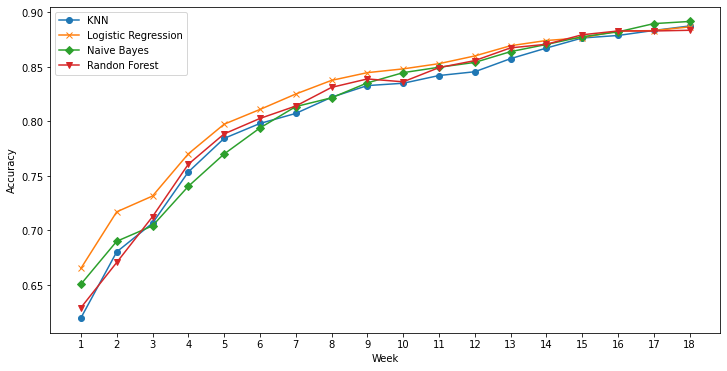
\includegraphics[scale=.6]{Resultados/binary_accuracy.png}
  	\textsf{\caption{Classifiers' accuracy (binary)}
  	\label{fig:ab}}
\end{figure}

\begin{figure}[htb]
	\centering
  	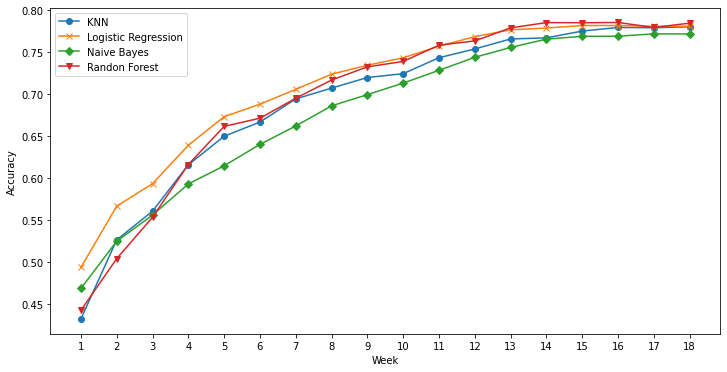
\includegraphics[scale=.6]{Resultados/3classes_accuracy.png}
  	\textsf{\caption{Classifiers' accuracy (3-class)}
  	\label{fig:a3c}}
\end{figure}

\begin{table}[htb]
\centering
\begin{tabular}{ccccccc} \hline
\multirow{2}{*}{\textbf{Week}} & \multicolumn{4}{c}{\textbf{Binary}} & \multicolumn{2}{c}{\textbf{3-class}} \\ 
 & \textbf{Accuracy} & \textbf{Precision} & \textbf{Recall} & \textbf{F-Measure} & \textbf{Accuracy} & \textbf{F-Measure} \\ \hline
1    & 66.51\% & 67.37\% & 80.97\% & 72.88\% & 49.32\% & 48.21\%   \\
2    & 71.70\% & 72.44\% & 81.70\% & 76.25\% & 56.63\% & 56.01\%   \\
3    & 73.15\% & 73.72\% & 81.99\% & 77.22\% & 59.31\% & 59.20\%   \\
4    & 77.03\% & 76.97\% & 84.97\% & 80.56\% & 63.89\% & 64.12\%   \\
5    & 79.74\% & 79.05\% & 87.30\% & 82.89\% & 67.30\% & 67.79\%   \\
6    & 81.10\% & 80.42\% & 88.06\% & 83.96\% & 68.79\% & 69.27\%   \\
7    & 82.51\% & 81.40\% & 89.58\% & 85.21\% & 70.56\% & 71.10\%   \\
8    & 83.76\% & 82.67\% & 90.22\% & 86.21\% & 72.36\% & 73.04\%   \\
9    & 84.47\% & 83.40\% & 90.60\% & 86.78\% & 73.44\% & 74.16\%   \\
10   & 84.82\% & 83.77\% & 90.80\% & 87.08\% & 74.32\% & 75.10\%   \\
11   & 85.30\% & 84.49\% & 90.72\% & 87.41\% & 75.71\% & 76.49\%   \\
12   & 86.01\% & 85.45\% & 90.78\% & 87.93\% & 76.85\% & 77.64\%   \\
13   & 86.94\% & 86.48\% & 91.27\% & 88.71\% & 77.66\% & 78.44\%   \\
14   & 87.42\% & 86.54\% & 92.21\% & 89.16\% & 77.87\% & 78.65\%   \\
15   & 87.67\% & 87.40\% & 91.56\% & 89.26\% & 78.17\% & 78.94\%   \\
16   & 88.30\% & 87.84\% & 92.23\% & 89.80\% & 78.17\% & 78.92\%   \\
17   & 88.33\% & 87.81\% & 92.38\% & 89.83\% & 78.07\% & 78.82\%   \\
18   & 88.67\% & 88.34\% & 92.32\% & 90.10\% & 78.09\% & 78.85\%   \\  \hline
\end{tabular}
\caption{Logistic regression model's performance}
\label{tab:lr}
\end{table}

\begin{figure}[htb]
	\centering
  	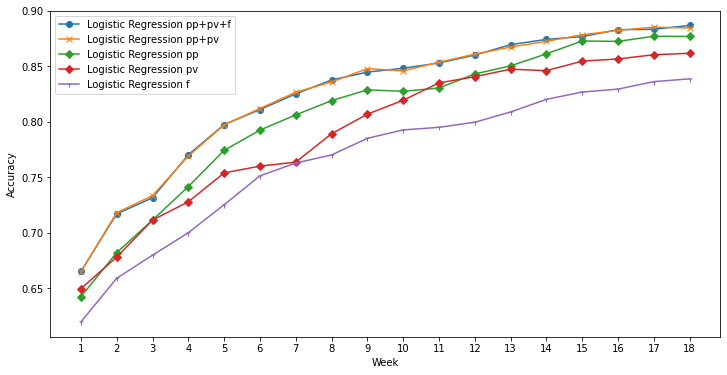
\includegraphics[scale=.6]{Resultados/lr_binary.png}
  	\textsf{\caption{Logistic regression model accuracy (binary)}
  	\label{fig:lrb}}
\end{figure}

\begin{figure}[!hb]
	\centering
  	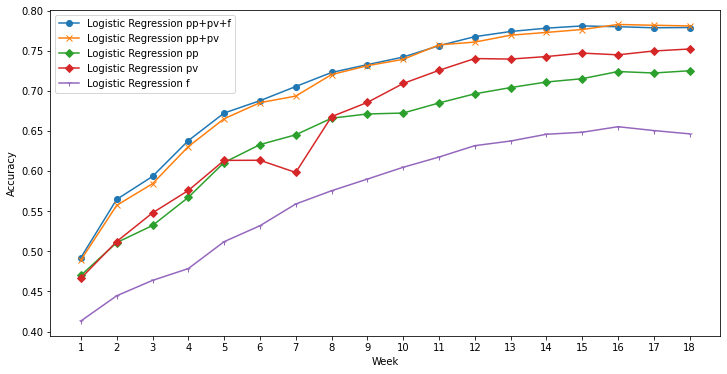
\includegraphics[scale=.6]{Resultados/lr_3classes.png}
  	\textsf{\caption{Logistic regression model accuracy (3-class)}
  	\label{fig:lr3c}}
\end{figure}


	\chapter{Logistic Regression models}
\label{ch:Models}

The Logistic Regression models obtained in the results of this work is shown in tables \ref{tab:model1} and \ref{tab:model2}. To clarify, $\pi(x)$ indicates the probability that a new instance $x$ belongs to the default class, which, in this case, is a student passing the course.

\begin{table}[htb]
\centering
\begin{tabular}{cc} \hline
\textbf{Week} & \textbf{Model} \\ \hline
1 & $logit[\pi(x)] = -2.1+0.14*pp_1+0.2*pv_1$ \\ \hline
2 & $logit[\pi(x)] =-3.31+0.1*pp_1+0.16*pp_2+0.06*pv_1+0.22*pv_2$ \\ \hline
3 & \begin{tabular}[c]{@{}c@{}}$logit[\pi(x)] =-3.5+0.07*pp_1+0.1*pp_2+0.13*pp_3+0.04*pv_1$\\$ +0.08*pv_2+0.19*pv_3$\end{tabular} \\ \hline
4 & \begin{tabular}[c]{@{}c@{}}$logit[\pi(x)] =-4.4+0.06*pp_1+0.08*pp_2+0.09*pp_3+0.17*pp_4$\\$ +0.02*pv_1+0.01*pv_2+0.08*pv_3+0.25*pv_4$\end{tabular} \\ \hline
5 & \begin{tabular}[c]{@{}c@{}}$logit[\pi(x)] =-4.3+0.05*pp_1+0.05*pp_2+0.06*pp_3+0.1*pp_4$\\$ +0.16*pp_5+0.03*pv_1+0.02*pv_2+0.05*pv_3+0.1*pv_4+0.17*pv_5$\end{tabular} \\ \hline
6 & \begin{tabular}[c]{@{}c@{}}$logit[\pi(x)] =-4.63+0.04*pp_1+0.04*pp_2+0.05*pp_3+0.08*pp_4$\\$ +0.12*pp_5+0.14*pp_6+0.02*pv_1+0.01*pv_2$\\$ +0.03*pv_3+0.07*pv_4+0.11*pv_5+0.11*pv_6$\end{tabular} \\ \hline
7 & \begin{tabular}[c]{@{}c@{}}$logit[\pi(x)] =-4.75+0.04*pp_1+0.03*pp_2+0.04*pp_3+0.06*pp_4$\\$ +0.09*pp_5+0.1*pp_6+0.14*pp_7+0.02*pv_1$\\$ +0.01*pv_2+0.03*pv_3+0.06*pv_4+0.08*pv_5+0.05*pv_6+0.12*pv_7$\end{tabular} \\ \hline
8 & \begin{tabular}[c]{@{}c@{}}$logit[\pi(x)] =-5.14+0.06*pp_1+0.02*pp_2+0.04*pp_3+0.04*pp_4$\\$ +0.07*pp_5+0.09*pp_6+0.11*pp_7+0.11*pp_8$\\$ +0.01*pv_1+0.01*pv_2+0.02*pv_3+0.06*pv_4$\\$ +0.06*pv_5-0.03*pv_6+0.03*pv_7+0.24*pv_8$\end{tabular} \\ \hline
9 & \begin{tabular}[c]{@{}c@{}}$logit[\pi(x)] =-5.29+0.05*pp_1+0.02*pp_2+0.04*pp_3$\\$ +0.04*pp_4+0.07*pp_5+0.07*pp_6+0.09*pp_7+0.08*pp_8$\\$ +0.1*pp_9+0.0*pv_1+0.01*pv_2+0.0*pv_3+0.06*pv_4$\\$ +0.05*pv_5-0.03*pv_6-0.01*pv_7+0.11*pv_8+0.23*pv_9$\end{tabular} \\ \hline
10 & \begin{tabular}[c]{@{}c@{}}$logit[\pi(x)] =-5.36+0.05*pp_1+0.01*pp_2+0.03*pp_3$\\$ +0.04*pp_4+0.06*pp_5+0.06*pp_6+0.08*pp_7+0.07*pp_8$\\$ +0.08*pp_9+0.06*pp_{10}+0.0*pv_1+0.02*pv_2$\\$ -0.01*pv_3+0.05*pv_4+0.05*pv_5$\\$ -0.03*pv_6-0.02*pv_7+0.08*pv_8+0.11*pv_9+0.21*pv_{10}$\end{tabular} \\ \hline
11 & \begin{tabular}[c]{@{}c@{}}$logit[\pi(x)] =-5.49+0.06*pp_1+0.01*pp_2+0.03*pp_3$\\$ +0.04*pp_4+0.07*pp_5+0.05*pp_6+0.08*pp_7+0.05*pp_8$\\$ +0.07*pp_9+0.03*pp_{10}+0.08*pp_{11}-0.0*pv_1$\\$ +0.01*pv_2-0.01*pv_3+0.05*pv_4+0.04*pv_5-0.03*pv_6$\\$ -0.02*pv_7+0.06*pv_8+0.06*pv_9+0.11*pv_{10}+0.25*pv_{11}$\end{tabular} \\ \hline
12 & \begin{tabular}[c]{@{}c@{}}$logit[\pi(x)] =-5.42+0.06*pp_1+0.01*pp_2+0.02*pp_3$\\$ +0.03*pp_4+0.07*pp_5+0.05*pp_6+0.09*pp_7+0.05*pp_8$\\$ +0.06*pp_9+0.01*pp_{10}+0.05*pp_{11}+0.08*pp_{12}$\\$ -0.01*pv_1+0.01*pv_2-0.01*pv_3+0.06*pv_4$\\$ +0.04*pv_5-0.04*pv_6-0.05*pv_7+0.04*pv_8$\\$ +0.05*pv_9+0.07*pv_{10}+0.15*pv_{11}+0.22*pv_{12}$\end{tabular} \\ \hline
\end{tabular}
\caption{Logistic Regression models (weeks 1-12)}
\label{tab:model1}
\end{table}

\begin{table}[htb]
\centering
\resizebox{12cm}{!}{%
\begin{tabular}{cc} \hline
\textbf{Week} & \textbf{Model} \\ \hline
13 & \begin{tabular}[c]{@{}c@{}}$logit[\pi(x)] =-5.25+0.04*pp_1+0.01*pp_2+0.01*pp_3$\\$ +0.02*pp_4+0.06*pp_5+0.04*pp_6+0.06*pp_7+0.04*pp_8$\\$ +0.05*pp_9+0.01*pp_{10}+0.04*pp_{11}+0.05*pp_{12}$\\$ +0.1*pp_{13}+0.0*pv_1+0.01*pv_2+0.0*pv_3+0.04*pv_4$\\$ +0.03*pv_5-0.02*pv_6-0.01*pv_7+0.03*pv_8+0.04*pv_9$\\$ +0.06*pv_{10}+0.09*pv_{11}+0.09*pv_{12}+0.14*pv_{13}$\end{tabular} \\ \hline
14 & \begin{tabular}[c]{@{}c@{}}$logit[\pi(x)] =-5.31+0.04*pp_1+0.02*pp_2+0.01*pp_3$\\$ +0.03*pp_4+0.06*pp_5+0.04*pp_6+0.05*pp_7+0.04*pp_8$\\$ +0.04*pp_9-0.0*pp_{10}+0.02*pp_{11}+0.03*pp_{12}$\\$ +0.07*pp_{13}+0.12*pp_{14}+0.0*pv_1+0.01*pv_2$\\$ +0.0*pv_3+0.03*pv_4+0.04*pv_5-0.02*pv_6$\\$ -0.02*pv_7+0.03*pv_8+0.04*pv_9+0.05*pv_{10}$\\$ +0.08*pv_{11}+0.07*pv_{12}+0.08*pv_{13}+0.12*pv_{14}$\end{tabular} \\ \hline
15 & \begin{tabular}[c]{@{}c@{}}$logit[\pi(x)] =-5.47+0.04*pp_1+0.01*pp_2+0.01*pp_3$\\$ +0.03*pp_4+0.06*pp_5+0.03*pp_6+0.06*pp_7+0.04*pp_8$\\$ +0.04*pp_9-0.01*pp_{10}+0.01*pp_{11}+0.02*pp_{12}$\\$ +0.05*pp_{13}+0.09*pp_{14}+0.09*pp_{15}+0.01*pv_1$\\$ +0.0*pv_2+0.0*pv_3+0.04*pv_4+0.03*pv_5$\\$ -0.02*pv_6-0.02*pv_7+0.02*pv_8+0.04*pv_9$\\$ +0.05*pv_{10}+0.07*pv_{11}+0.05*pv_{12}$\\$ +0.05*pv_{13}+0.08*pv_{14}+0.12*pv_{15}$\end{tabular} \\ \hline
16 & \begin{tabular}[c]{@{}c@{}}$logit[\pi(x)] =-5.82+0.05*pp_1+0.01*pp_2+0.01*pp_3$\\$ +0.04*pp_4+0.07*pp_5+0.04*pp_6+0.06*pp_7+0.05*pp_8$\\$ +0.04*pp_9-0.02*pp_{10}+0.0*pp_{11}+0.0*pp_{12}$\\$ +0.04*pp_{13}+0.08*pp_{14}+0.08*pp_{15}+0.07*pp_{16}$\\$ +0.01*pv_1+0.0*pv_2+0.0*pv_3$\\$ +0.06*pv_4+0.05*pv_5-0.05*pv_6$\\$ -0.05*pv_7+0.01*pv_8+0.06*pv_9+0.06*pv_{10}$\\$ +0.09*pv_{11}+0.05*pv_{12}+0.03*pv_{13}+0.05*pv_{14}$\\$ +0.11*pv_{15}+0.11*pv_{16}$\end{tabular} \\ \hline
17 & \begin{tabular}[c]{@{}c@{}}$logit[\pi(x)] =-5.56+0.04*pp_1+0.01*pp_2+0.01*pp_3$\\$ +0.03*pp_4+0.05*pp_5+0.03*pp_6+0.05*pp_7+0.04*pp_8$\\$ +0.04*pp_9-0.02*pp_{10}+0.01*pp_{11}+0.0*pp_{12}$\\$ +0.03*pp_{13}+0.06*pp_{14}+0.06*pp_{15}+0.04*pp_{16}$\\$ +0.1*pp_{17}+0.01*pv_1+0.01*pv_2$\\$ +0.0*pv_3+0.04*pv_4+0.04*pv_5-0.02*pv_6$\\$ -0.02*pv_7+0.02*pv_8+0.04*pv_9+0.05*pv_{10}$\\$ +0.07*pv_{11}+0.05*pv_{12}+0.04*pv_{13}+0.04*pv_{14}$\\$ +0.07*pv_{15}+0.06*pv_{16}+0.08*pv_{17}$\end{tabular} \\ \hline
18 & \begin{tabular}[c]{@{}c@{}}$logit[\pi(x)] =-4.62+0.02*pp_1+0.01*pp_2+0.01*pp_3$\\$ +0.02*pp_4+0.03*pp_5+0.02*pp_6+0.03*pp_7+0.03*pp_8$\\$ +0.03*pp_9+0.01*pp_{10}+0.02*pp_{11}+0.02*pp_{12}$\\$ +0.03*pp_{13}+0.04*pp_{14}+0.04*pp_{15}+0.04*pp_{16}$\\$ +0.05*pp_{17}+0.06*pp_{18}+0.01*pv_1+0.01*pv_2$\\$ +0.01*pv_3+0.02*pv_4+0.02*pv_5+0.01*pv_6$\\$ +0.01*pv_7+0.02*pv_8+0.03*pv_9+0.03*pv_{10}$\\$ +0.04*pv_{11}+0.03*pv_{12}+0.03*pv_{13}+0.03*pv_{14}$\\$ +0.04*pv_{15}+0.04*pv_{16}+0.04*pv_{17}+0.05*pv_{18}$\end{tabular}\\ \hline
\end{tabular}%
}
\caption{Logistic Regression models (weeks 13-18)}
\label{tab:model2}
\end{table}
	
	% Anexo A (arquivo Includes/AnexoA)
	%% Anexo
\anexo
\chapter{Anexo A}



\end{document}
